\documentclass[journal,12pt,onecolumn]{IEEEtran}
\usepackage{cite}
\usepackage{caption}
\usepackage{graphicx}
\usepackage{amsmath,amssymb,amsfonts,amsthm}
\usepackage{algorithmic}
\usepackage{graphicx}
\usepackage{textcomp}
\usepackage{xcolor}
\usepackage{txfonts}
\usepackage{listings}
\usepackage{enumitem}
\usepackage{mathtools}
\usepackage{gensymb}
\usepackage{comment}
\usepackage[breaklinks=true]{hyperref}
\usepackage{tkz-euclide} 
\usepackage{listings}
\usepackage{gvv}
%\def\inputGnumericTable{}                                 
\usepackage[latin1]{inputenc} 
\usetikzlibrary{arrows.meta, positioning}
\usepackage{xparse}
\usepackage{color}                                            
\usepackage{array}                                            
\usepackage{longtable}                                       
\usepackage{calc}                                             
\usepackage{multirow}
\usepackage{multicol}
\usepackage{hhline}                                           
\usepackage{ifthen}                                           
\usepackage{lscape}
\usepackage{tabularx}
\usepackage{array}
\usepackage{float}

\usepackage{float}
%\newcommand{\define}{\stackrel{\triangle}{=}}
\theoremstyle{remark}
\usepackage{circuitikz}
\captionsetup{justification=centering}
\usepackage{tikz}

\title{Matrices in Geometry 2.4.34}
\author{EE25BTECH11037 - Divyansh}
\begin{document}
\vspace{3cm}
\maketitle
{\let\newpage\relax\maketitle}
\textbf{Question: }
What type of quadrilateral do the points $\vec{A}\brak{2,-2}$, $\vec{B}\brak{7,3}$, $\vec{C}\brak{11,-1}$ and $\vec{D}\brak{6,-6}$ taken in that order, form?


\textbf{Given: } $\vec{A}\myvec{2\\-2}$, $\vec{B}\myvec{7\\3}$, $\vec{C}\myvec{11 \\ -1}$ and $\vec{D}\myvec{6 \\ -6}$.
 

\begin{align}
    \vec{B}- \vec{A}=\myvec{5 \\ 5} \\
    \vec{C}- \vec{B}=\myvec{4 \\ -4} \\
    \vec{D}- \vec{C}=\myvec{-5 \\ -5} \\
    \vec{A}- \vec{D}=\myvec{-4 \\ 4} \\
    \text{Checking opposite sides, } \ \vec{D}-\vec{C}=-\brak{\vec{A}-\vec{B}} \text{ and } \vec{A}-\vec{D}=-\brak{\vec{B}-\vec{C}}
\end{align}
Each pair of opposite sides are parallel and equal in length; this implies that the quadrilateral is a parallelogram.\\
Now, checking for right angle, we check for inner product.
\begin{align}
 \brak{\vec{B}- \vec{A}}^{\top} \brak{\vec{C}- \vec{B}}=\myvec{5 & 5}\myvec{4 \\ -4}=0
\end{align}
This implies that the angle at $\vec{B}$ is one right angle. A parallelogram with a right angle is a rectangle.\\
Checking for a square:\\
The give quadrilateral is a square if its diagonals are orthogonal,
\begin{align}
\brak{\vec{C}- \vec{A}}^{\top} \brak{\vec{D}- \vec{B}}=\myvec{9 & 1}\myvec{-1 \\ -9}=-18
\end{align}
We can see that $\brak{\vec{C}- \vec{A}}^{\top} \brak{\vec{D}- \vec{B}}$ is $\neq 0$, that is, the diagonals are not orthogonal and therefore the quadrilateral $\vec{A}\vec{B}\vec{C}\vec{D}$ cannot be a square.\\
$\therefore$ The quadrilateral $\vec{A}\vec{B}\vec{C}\vec{D}$ is a rectangle.



\begin{figure}[H]
    \centering
    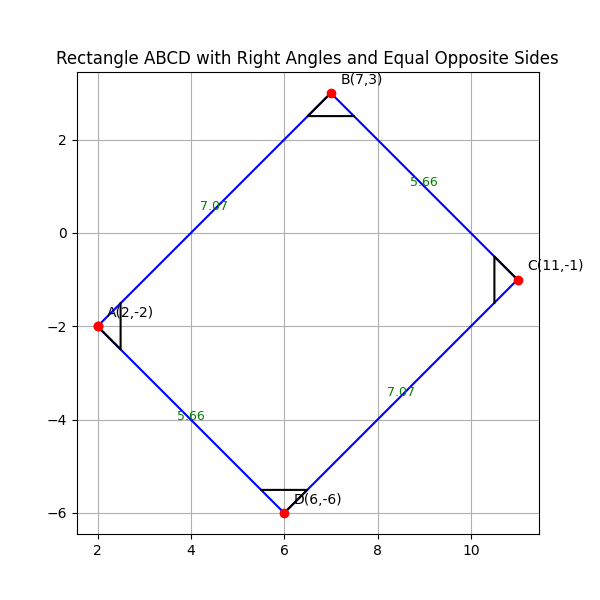
\includegraphics[width=1\columnwidth]{figs/1.png}
    \caption{Plot for 2.4.34}
    \label{fig:placeholder}
\end{figure}
\end{document}